\chapter{Statistics}\label{chapter:stats}

This chapter provides an overview of the statistics used in LingPipe
as well as the statistical utilities provided as classes and methods
by LingPipe.  Without the space to repeat an entire calculus, matrix
and math stats curriculum, we use this appendix more as a reminder for
the definitions we use in the book.

\section{Useful Functions}


\subsection{Logarithms and Exponents}

The exponential function $\exp(x)$ is defined as the unique non-zero
solution to the differential equation $f' = f$.  Thus we have
%
\begin{equation}
\frac{d}{dx}\exp(x) = \exp(x)
\ \ \ \ \ \mbox{and} \ \ \ \ \ 
\int \exp(x) \ dx = \exp(x).
\end{equation}

The exponential function may be applied to any real number, but its
value is always positive.  The exponential function has some
convenient properties, such as
%
\begin{equation}
\exp(a + b) = \exp(a) \times \exp(b), \mbox{ and}
\end{equation}
%
\begin{equation}
\exp(a \times b) = \exp(a)^b.
\end{equation}

The natural logarithm, $\log x$ is defined as the inverse of $\exp(x)$,
so that for all $x \in (-\infty,\infty)$ and all $y \in (0,\infty)$ we have
%
\begin{equation}
\log \exp(x) = x
\ \ \ \ \ \mbox{and} \ \ \ \ \ 
\exp(\log y) = y.
\end{equation}
%

Logarithms convert multiplication into addition and exponentiation
into multiplication, with
%
\begin{equation}
\log (x \times y) = \log x + \log y, \mbox{ and}
\end{equation}
%
\begin{equation}
\log x^y = y \log x.
\end{equation}



\subsection{The Factorial Function}\label{section:stats-factorial}

The factorial function computes the number of different ordered
permutations there are of a list of a given (non-negative) number of
distinct objects.  The factorial function is written $n!$
and defined for $n \in \nats$ by
%
\begin{equation}
n! = 1 \times 2 \times \cdots \times n = \prod_{m=1}^n m.
\end{equation}
%
The convention is to set $0! = 1$ so that the boundary conditions of
definitions like the one we provided for the binomial coefficient work
out properly.


\subsection{Binomial Coefficients}\label{section:stats-binomial-coefficient}

The binomial coefficient has many uses.  We're mainly interested in
combinatorics, so we think of it as providing the number of ways to
select a subset of a given size from a superset of a given size.  The
binomial coefficient is written ${m choose n}$, prounced ``$m$
choose $n$,'' and defined for $m, n \in \nats$ with $n \geq m$ by
%
\begin{equation}
{n \choose m} = \frac{n!}{m! \ (n-m)!}.
\end{equation}


\subsection{The $\Gamma$ Function}\label{section:stats-gamma-function}

The $\Gamma$ function is the complex generalization of the factorial
function (see \refsec{stats-factorial}).  It is written $\Gamma(x)$, 
and we're only concerned with real $x \in [0,\infty)$, where its value
is defined by 
%
\begin{equation}
\Gamma(x) = \int_0^{\infty} t^{x-1} \ \exp(-t) \ dt.
\end{equation}
%
In general, we have
%
\begin{equation}
\Gamma(x+1) = x \ \Gamma(x).
\end{equation}
%
Because we have $\Gamma(1) = 1$, we also have for all $n \in \nats, n > 0$, 
%
\begin{equation}
\Gamma(n) = (n-1)!.
\end{equation}


\section{Discrete Probability Distributions}


\subsection{Binomial Distribution}

\subsubsection{Distribution}

The binomial distribution is parameterized by a chance-of-success
parameter $\theta \in [0,1]$ and a number-of-trials parameter $N \in
\nats$.  If a random variable $X$ has a binomial distribution with
parameters $\theta$ and $N$, we write $X \sim \dbin{\theta}{N}$.  The
probability distribution for $X \sim \dbin{\theta}{N}$ is given by 
%
\begin{equation}
p_X(n) = {N \choose n} \ \theta^{n} \ (1-\theta)^{N-n}.
\end{equation}
%
%

\subsubsection{Variance}\label{section:stats-binomial-variance}

The variance and standard deviation of a binomially-distributed random
variable $X \sim \dbin{\theta}{N}$ are given by
%
\begin{equation}
\hfill
\var{X} = \frac{\theta (1 - \theta)}{N} 
\hspace*{0.25in}
\mbox{and}
\hspace*{0.25in}
\sd{X} = \sqrt{\frac{\theta (1 - \theta)}{N}}.
\hfill
\end{equation}
%

We are often more interested in the percentage of the $N$ trials that
resulted in success, which is given by the random variable $X/N$ (note
that $N$ is a constant here).  The variable $X/N$ is scaled to be
between 0 and 1.  With large $N$, $X/N$, will be approximately equal
to $\theta$ for almost every trial.  The variance and standard
deviation of $X/N$ are derived in the usual way, by dividing by the
constant $N$,
%
\begin{equation}
\var{X/N} = \theta (1 - \theta) 
\hspace*{0.25in}
\mbox{and}
\hspace*{0.25in}
\sd{X/N} = \sqrt{\theta (1-\theta)}.
\end{equation}



\section{Continuous Probability Distributions}

\subsection{Normal Distribution}\label{section:stats-normal-distribution}



\subsection{$\chi^2$ Distribution}\label{section:stats-chi-squared-distribution}

The $\chi^2$ distribution with $n$ degrees of freedom arises as the
sum of the squares of $n$ independent unit normal distributions (see
\refsec{stats-normal-distribution}).  In symbols, if $X_n \sim \dnorm(0,1)$
for $n \in 1{:}N$, then 
%
\begin{equation}
Y = \sum_{n=1}^N X_n^2
\end{equation}
%
has a $\chi^2$ distribution with $N$ degrees of freedom.

If a variable $X$ has a $\chi^2$ distribution with $N$ degrees of
freedom, we write $X \sim \dchisq{N}$.  The probability distribution
for $X$ is defined for $x \in [0,\infty)$ by
%
\begin{equation}
p_X(x) = \frac{1}{2^{N/2} \ \Gamma(n/2)} \ x^{N/2-1} \ \exp(-x/2).
\end{equation}
%

If $X \sim \dchisq{N}$, then the mean, variance and standard deviation of $X$ are
%
\begin{equation}
\expect{X} = N,
\ \ \ \ \ 
\var{X} = 2n, \mbox{ and}
\ \ \ \ \  
\sd{X} = \sqrt{2n}.
\end{equation}


\section{Contingency Tables}

A contingency table is an $M \times N$ matrix $C$ of counts
\ie{$C_{m,n} \in \nats$}.  A generic contingency table is shown in
\reffig{stats-generic-contingency-table}.
%
\begin{figure}
\begin{center}
\begin{tabular}{c|cccc||c}
& 1 & 2 & $\cdots$ & $N$ & \tblhead{Total}
\\ \hline
1 & $C_{1,1}$ & $C_{1,2}$ & $\cdots$ & $C_{1,N}$ & $C_{1,+}$
\\
2 & $C_{2,1}$ & $C_{2,2}$ & $\cdots$ &  $C_{2,N}$ & $C_{2,+}$
\\
$\vdots$ & $\vdots$ & $\vdots$ & $\ddots$ & $\vdots$ & $\vdots$
\\
$M$ & $C_{M,1}$ & $C_{M,2}$ & $\cdots$ & $C_{M,N}$ & $C_{M,+}$
\\
\hline \hline
\tblhead{Total} & $C_{+,1}$ & $C_{+,2}$ & $\cdots$ & $C_{+,N}$& $C_{+,+}$
\end{tabular}
\end{center}
\caption{A generic $M \times N$ contingency table $C$.  Each entry
  $C_{m,n}$ represents a cell count.  The values along the bottom and
  on the right side are totals of their respective columns and rows.
  The value in the lower right corner is the total count in the
  table.}\label{fig:stats-generic-contingency-table}
\end{figure}
%
We use the notation $C_{m,+}$ for the sum of the values in row $m$,
$C_{+,n}$ for the sum of the values in column $n$, and and $C_{+,+}$
for the sum of the entire table.  These values are defined by
%
\begin{equation}
C_{m,+} = \sum_{n=1}^N C_{m,n}, 
\ \ \ \ \ \
C_{+,n} = \sum_{m=1}^M C_{m,n}, \mbox{ and}
\ \ \ \ \ \  
C_{+,+} = \sum_{m=1}^M \sum_{n=1}^N C_{m,n}.
\end{equation}



\subsection{$\chi^2$ Tests of Independence}\label{section:stats-chi-square-independence}

The $\chi^2$ distribution may be used to test the null hypothesis that
that a pair of categorical random variables are generated
independently.

Suppose we have $K$ independent and identically distributed (i.i.d.)
pairs $A_k, B_k$ of categorical random variables taking values $A_k
\in 1{:}M$ and $B_k \in 1{:}N$.  Being identically distributed means
the pairs share distributions, so that
%
\begin{equation}
p\!_{A_i,B_i} = p\!_{A_j,B_j} \mbox{ for } i, j \in 1{:}K.
\end{equation}
%
Independence requires that the value of the pair $A_i,B_i$ is
independent of the value of the pair $A_j,B_j$ if $i \neq j$.

So far, we have allowed for the possibility that $A$ and $B$ are not
independent of each other.  If $A_k$ and $B_k$ are independent, then
%
\begin{equation}
p\!_{A_k,B_k}(x,y) = p\!_{A_k}(x) \times p_{B_k}(y).
\end{equation}
%
Because we've assumed the $A_k,B_k$ pairs are i.i.d., they share
distributions and hence are either all independent or all
non-independent.

We define an $M \times N$ contingency table $C$ by setting
%
\begin{equation}
C_{m,n} = \sum_{k=1}^K \indicator{A_k = m, B_k = n}.
\end{equation}
%
That is, $C_{m,n}$ is the number of times $A_i$ was $m$ and $B_i$ was
$n$.  Note that $C$ is a matrix random variable defined as a function
of the random variables $A$ and $B$.

Given a contingency table $C$, we can estimate the marginal
distributions $p_A(m)$ and $p_B(n)$ by maximum likelihood using the
observed counts in $C$.  Because $p_A$ and $p_B$ are multinomials, we
assume $p_A = \dbern{\theta}$ and $p_B = \dbern{\phi}$.  The
maximum likelihood estimates $\theta^*, \phi^*$ of $\theta,\phi$
given $C$ are
%
\begin{equation}
\theta^*_m = \frac{C_{m,+}}{C_{+,+}} 
\ \ \ \ \ \mbox{and} \ \ \ \ \ 
\phi^*_n = \frac{C_{+,n}}{C_{+,+}}.
\end{equation}

Pearson's independence test involves the statistic $X^2$, which is
defined in terms of $C$ by
%
\begin{equation}
X^2 
= \sum_{m=1}^M \ \sum_{n=1}^N 
  \frac{(C_{m,n} - E_{m,n})^2}
       {E_{m,n}}
\end{equation}
%
where $E_{m,n}$ is the expected value of $C_{m,n}$ (given our
estimates $\theta^*$ and $\phi^*$) if $A$ and $B$ are independent,
%
\begin{equation}
E_{m,n} = C_{+,+} \ \times \ \theta^*_m \ \times \ \phi^*_n.
\end{equation}

If $A_k$ and $B_k$ are independent, the distribution of the statistic
$X^2$ is approximately $\chi^2$ with $(M-1) \times (N-1)$ degrees of
freedom (see \refsec{stats-chi-squared-distribution}).%
%
\footnote{The proof is too complex, but we provide some hints as to
  its form.  We have $MN$ cells, so have $MN-1$ degrees of freedom, of
  which we lose $M-1$ and $N-1$ because we are estimating $\theta^*$
  and $\phi^*$, which have one less than their dimensionality degrees
  of freedom, $M-1$ and $N-1$, for a total of $MN-1 - (M + N -2) =
  (M-1)(N-1)$ degrees of freedom (again, asymptotically).  Because the
  $C_{m,n}$ are binomially distributed with success probability
  $\theta^*_m \times \phi^*_n$ and $C_{+,+}$ trials, the central limit
  theorem ensures asymptotic normality of $C_{m,n}$ as $C_{+,+}$
  grows.  The mean or expected value of the binomial is $E_{m,n}$, and
  a binomial's variance is equal to its mean.  Rewriting the term
  inside the summation in the definition of the $X^2$ statistic as
  $((C_{m,n} - E_{m,n})/\sqrt{E_{m,n}})^2$ reveals that its just a
  squared z-score.}
%
The usual rule of thumb is that the approximation is reliable if each
of the expected counts $E_{m,n}$ is at least 5.

As usual, the classical hypothesis test rejects the null hypothesis with
$p$-value $\alpha$ if the value of the test statistic $X^2$ is outside
of the central and columns are independent if the $X^2$ statistic is
outside of the central probabiilty interval of $1-p$.

\subsection{Further Contingency and Association Statistics}

\subsubsection{Pearson's Mean Square Contingency}
Dividing Pearson's $\chi^2$ statistic $X^2$ by the number of cases
yields Pearson's $\varphi^2$ statistic.
%
\begin{equation}
\varphi^2 =\frac{X^2}{C_{+,+}}
\end{equation}
%
The $\varphi^2$ statistic is known as the mean square contingency for
the table $C$.  As with $X^2$, larger values indicate more contingency.

\subsubsection{Cramér's Degree of Association}

Cramér's V statistic%
%
\footnote{H. Cramér. 1999. {\it Mathematical Methods of
    Statistics}. Princeton University Press.}
%
is designed to measure the degree of association between the
rows and columns in a general contingency table.   The square of
$V$ is defined by dividing $\varphi^2$ by the minimum of the number
of rows and columns minus 1,
%
\begin{equation}
V^2 = \frac{\varphi^2}{\min(M,N)-1}.
\end{equation}
%
Obviously, the definition only makes sense if $M,N \geq 2$, and if
$M=2$ or $N=2$, $V^2$ reduces to $\varphi^2$.  As with $\varphi^2$ and
$X^2$, larger values of $V^2$ indicate stronger associations.

\subsubsection{Goodman And Kruskal's Index of Predictive Association}

Goodman and Kruskal defined an asymmetric measure of predictive
association which they called $\lambda_B$.%
%
\footnote{Goodman and Kruskal wrote three papers analyzing
  cross-classified data such as is found in contingency matrices,
  starting with Goodman, L.~A. and W.~H.~Kruskal, 1954, Measures of
  association for cross classifications, Part I, {\it Journal of the
    American Statistical Association} {\bf 49}:732–-764.  With the
  same journal and title, Part II was
  published in 1959 in volume {\bf 53}, pages 123--163, and Part III
  in 1963 in volumne {\bf 58}, pages 310--364.}
%
The value of $\lambda_B$ is (an estimate of) the reduction in error
likelihood from knowing the response category and using it to predict
the reference category.  It takes on values between 0 and 1, with
higher values being better, 0 indicating independence and 1 perfect
assocaition.  

Given our $M \times N$ confusion matrix $C$, Goodman and Kruskal's
index of predictive association $\lambda_B$ is defined by
%
\begin{equation}
\lambda_A 
= \frac{\left(\sum_n R_n\right) - S}
       {C_{+,+} - S}
\end{equation}
%
where $S$ and $R_n$ are defined by 
%
\begin{equation}
S = \max_n \ C_{+,n}
\ \ \ \ \ \mbox{and} \ \ \ \ \
R_n = \max_m \ C_{n,m}.
\end{equation}
%
These statistics are unusual in using the maximum rather than
matching.  Dividing through by $C_{+,+}$ reveals a structure very much
like the $\kappa$ statistic (see \refsec{stats-kappa}), with $e$
replaced by $S/C_{+,+}$ and with $a$ replaced by $\sum_n R_n /
C_{+,+}$.

The $\lambda_B$ statistic is not symmetric between the rows and
columns.  If we transpose the matrix and compute the same statistic,
we get $\lambda_Ap$.


\subsection{Information-Theoretic Measures}

If we use the counts in $C$ to estimate probability distributions
using maximum likelihood, we may use any of the information-theoretic
measures available to compare distributions (see
\refsec{stats-information-theory} for definitions).  

For example, suppose we define random variables $X$ and $Y$ for the
rows and columns, with joint distribution given by the maximum
likelihood estimate given the contingency table $C$, which entails
%
\begin{equation}
p_{X,Y}(m,n) = \frac{C_{m,n}}{C_{+,+}}.
\end{equation}
%
Given this defintion, the marginal distributions for $X$ and $Y$ are
%
\begin{equation}
p_X(m) = \frac{C_{m,+}}{C_{+,+}}
\ \ \ \ \ \mbox{and} \ \ \ \ \
p_Y(n) = \frac{C_{+,n}}{C_{+,+}}.
\end{equation}
%
The conditional distributions for $X$ given $Y$ and vice-versa are
%
\begin{equation}
p_{X|Y}(m|n) = \frac{C_{m,n}}{C_{m,+}}
\ \ \ \ \ \mbox{and} \ \ \ \ \
p_{Y|X}(m|n) = \frac{C_{m,n}}{C_{+,n}}.
\end{equation}

With all of these definitions in hand, we can easily compute the
various information theoretic measures, which are defined in
\refsec{stats-information-theory}.

For instance, we can compute the entropy corresponding to the rows of
the contingency table as $\entropy{X}$ and to the columns as
$\entropy{Y}$.  We can also compute the KL-divergences, symmetrized
divergences and Jensen-Shannon divergence based on the marginal
distributions $p_X$ and $p_Y$ implied by the contingency table.

With the joint and conditional estimates, we can tabulate the joint
entropy $\entropy{X,Y}$, conditional entropies $\condentropy{X}{Y}$
and $\condentropy{Y}{X}$, as well as and mutual information
$\mutualinfo{X}{Y}$.


\subsection{Confusion Matrices}

A confusion matrix is just a square ($N \times N$) contingency table
where the variable represented by the rows and columns has the same
set of categorical outcomes.  Confusion matrices are often used to
evaluate classifiers, taking the rows to represent reference
categories and columns to represent system responses.

There is a wide range of statistics that have been applied to
evaluating the performance of classifiers using confusion matrices.

\subsection{$\kappa$ Statistics for Chance-Adjusted Agreement}\label{section:stats-kappa}

Suppose we have an $N \times N$ confusion matrix $C$.  

Cohen's $\kappa$ statistic%
\footnote{Cohen, Jacob. 1960. A coefficient of agreement for nominal
  scales. {\it Educational And Psychological Measurement} {\bf
    20}:37-46.}
%
is defined by
%
\begin{equation}
\kappa = \frac{a - e}{1 - e},
\end{equation}
%
where
%
\begin{equation}
a = \frac{\sum_{n=1}^N C_{n,n}}{C_{+,+}}
\ \ \mbox{ and } \ \ 
e = \sum_{n=1}^N \theta^*_n \ \times \ \phi^*_n = \frac{E_{n,n}}{C_{+,+}}.
\end{equation}
%
In words, $a$ is the percentage of cases in which there was agreement,
in other words the total accuracy, and $e$ is the expected accuracy if
the reference and response are independent.

Siegel and Castellan's $\kappa$ statistic%
\footnote{Siegel, Sidney and N.~John Castellan, Jr. 1988.  {\it
    Nonparametric Statistics for the Behavioral Sciences}. McGraw
  Hill.}
%
has the same definitional form as Cohen's, but the calculation of the
expectation is based on averaging the reference and response to define
%
\begin{equation}
e = \sum_{n=1}^N \left( \frac{\theta^*_n + \phi^*_n}{2} \right)^2.
\end{equation}

Byrt et al.'s $\kappa$ statistic%
%
\footnote{Byrt, Ted, Janet Bishop and John B. Carlin. 1993. Bias,
  prevalence, and kappa. {\it Journal of Clinical Epidemiology}
  {\bf 46}(5):423--429.}
%
completely ignores the adjustment for
category prevalence found in $e$, taking an arbitrary 50\% chance of
agreement, corresponding to $e=1/2$, and resulting in a definition of
$\kappa = 2a - 1$.



\subsection{Sensitivity-Specificity Matrices}

A sensitivity-specificity matrix is a $2 \times 2$ confusion matrix
where the binary categories are distinguished as ``positive'' and
``negative'' (or ``true'' and ``false'' or ``accept'' and ``reject'').
The cells have conventional names in a sensitivity-specificy matrix,
which we show in \reffig{generic-sensitivity-specificity-matrix}.
%
\begin{figure}
\begin{center}
\begin{tabular}{rr|cc}
\multicolumn{2}{c}{ } & \multicolumn{2}{c}{\tblhead{\bfseries Response}}
\\
\multicolumn{2}{c|}{ } & \tblhead{Positive} & \tblhead{Negative}
\\
\cline{2-4}
\multirow{2}{0.15\textwidth}{\tblhead{\bfseries Reference}}
& \tblhead{Positive} & TP & FN
\\
& \tblhead{Negative} & FP & TN

\end{tabular}
\end{center}
\caption{A generic sensitivity-specificity matrix is a $2 \times 2$
  confusion matrix with columns and rows labeled with ``positive'' and
  ``negative.''.  The code P (positive) is assigned to reference
  positives and N (negative) to reference negatives, with T (true)
  assigned to correct responses and F (false) to incorrect
  responses.}\label{fig:generic-sensitivity-specificity-matrix}
\end{figure}
%
The true positives (TP), false positives (FP) are for correct and
incorrect responses when the reference category is positive, and true
negative (TN) and false negative (FN) for correct and incorrect
responses when the reference category is negative.  False positives
are also known as type-I errors or false alarms, and false negatives
as misses or type-II errors.

\subsubsection{Precision and Recall}

For search and many classification evaluations, precision and recall
are the most commonly reported metrics.  Given a
sensitivity-specificity matrix, precision and recall are calculated as
%
\begin{equation}
\mbox{precision} = \frac{TP}{TP+FP}
\ \ \ \ \ \mbox{and} \ \ \ \ \ 
\mbox{recall} = \frac{TP}{TP+FN}.
\end{equation}
%
Precision is the percentage of positive responses
($\mbox{TP}+\mbox{FN}$) that are correct, whereas and recall the
percentage of positive reference items ($\mbox{TP}+\mbox{FP}$) that
were assigned a positive response.  Looking at the matrix, we see that
recall is based on the top row and precision on the left column.  In
the next sections, we'll fill in the dual statistics.

Precision is sometimes called positive predictive accuracy, because
it's the accuracy for items that get a positive prediction.

\subsubsection{Sensitivity and Specificity}

Sensitivity and specificity are more commonly used to evaluate
sensitivity-specificity matrices (hence the name we gave them). 
These are defined by 
%
\begin{equation}
\mbox{sensitivity} = \frac{TP}{TP+FN}
\ \ \ \ \ \mbox{and} \ \ \ \ \ 
\mbox{specificity} = \frac{TN}{TN+FP}
\end{equation}
%
Sensitivity is the same statistic as recall, being based on the top
row of the matrix.  One minus specificity is sometimes called fallout.

The easiest way to think of sensitivity and specificity is as
accuracies on reference positives ($\mbox{TP}+\mbox{FN}$) and
reference negatives ($\mbox{TN}+\mbox{FP}$), respectively.

Sensitivity and specificity are based on all four cells of the matrix,
whereas precision and recall do not use the true negative count.

\subsubsection{Transpose Duals and Rejection Precision}

If we transpose the roles of the reference and response, we swap FN
and FP counts, but TP and TN remain the same.  Precision becomes
recall and vice versa in the transposed matrix.  Specificity, on
the other hand, does not have a dual defined yet.  To complete the
picture, we introduce a statistic we call rejection precision,
which is defined by
%
\begin{equation}
\mbox{rejection-precision}
= \frac{TN}{TN+FP}.
\end{equation}
%
This is the percentage of negative responses that are truly negative,
and could also be called negative predictive accuracy.  

To use terminology to match rejection precision, we could call
specificity rejection recall.  Rejection precision and rejection
recall swap when the matrix is transposed in the same way as precision
and recall.  The dualities are clearest when viewed in table form,
as laid out in \reffig{precision-recall-duality}.
%
\begin{figure}
\begin{center}
\small
\begin{tabular}{r|c|c}
\multicolumn{3}{l}{\tblhead{\bfseries Recall}}
\\
\multicolumn{1}{c}{}  & \tblhead{Pos} & \tblhead{Neg}
\\ \cline{2-3}
\tblhead{Pos} & {\bfseries +} & {\bfseries --}
\\ \hline
\tblhead{Neg} & & 
\end{tabular}
%
\hfill
%
\begin{tabular}{r|c|c}
\multicolumn{3}{l}{\tblhead{\bfseries Precision}}
\\
\multicolumn{1}{c}{}  & \tblhead{Pos} & \tblhead{Neg}
\\ \cline{2-3}
\tblhead{Pos} & {\bfseries +} & 
\\ \hline
\tblhead{Neg} & {\bfseries --} & 
\end{tabular}
%
\hfill
%
\begin{tabular}{r|c|c}
\multicolumn{3}{l}{\tblhead{\bfseries Rej.~Recall}}
\\
\multicolumn{1}{c}{}  & \tblhead{Pos} & \tblhead{Neg}
\\ \cline{2-3}
\tblhead{Pos} & & 
\\ \hline
\tblhead{Neg} & {\bfseries --} & {\bfseries +}
\end{tabular}
%
\hfill
%
\begin{tabular}{r|c|c}
\multicolumn{3}{l}{\tblhead{\bfseries Rej.~Precicision}}
\\
\multicolumn{1}{c}{}  & \tblhead{Pos} & \tblhead{Neg}
\\ \cline{2-3}
\tblhead{Pos} & & {\bfseries --}
\\ \hline
\tblhead{Neg} & & {\bfseries +}
\end{tabular}
\end{center}
\caption{A graphical illustration of the transposition dualities
  involved in the definitions of recall (sensitivity) and precision
  (positive predictive accuracy) and in the definitions of rejection
  recall (specificity) and rejection precision (negative predictive
  accuracy).  The symbol {\bfseries +} indicates successfull attempts
  and {\bfseries --} failed attempts.  The statistic labeing the table
  is calculated as the percentage of attempts that were successful
  based on the value of the cells (see
  \reffig{generic-sensitivity-specificity-matrix}).}\label{fig:precision-recall-duality}
\end{figure}

\subsubsection{$F$ Measure}

A common measure used in information retrieval research is $F$ measure,
which is defined as the harmonic mean of precision and recall,
%
\begin{equation}\label{eq:f-measure}
F
= \left( \mbox{precision}^{-1} + \mbox{recall}^{-1} \right)^{-1}
= \frac{2 \times \mbox{precision} \times \mbox{recall}}
         {\mbox{precision} + \mbox{recall}}.
\end{equation}

Sometimes, this measure is generalized with a weighting $\beta$
to be
%
\begin{equation}
F_{\beta} = \frac{(1 + \beta^2) \times \mbox{precision} \times \mbox{recall}}
                {\mbox{recall} + (\beta^2 \times \mbox{precision})}.
\end{equation}
%
With this generalization, the original $F$ measure in
\refeq{f-measure} corresonds to the generalized $F$ measure with
$\beta=1$.  

$F$ measure has the property, because it is based on a harmonic mean,
of always being less than the simple average of precision and recall.

For some reason, $F$ measure is the only commonly applied statistic
based on the harmonic mean.  You don't see people compute the harmonic
mean of sensitivity and specificity or of rejection recall and
rejection precision.

\subsubsection{Jaccard Similarity Coefficient}

The Jaccard similarity coefficient%
%
\footnote{Jaccard, Paul. 1901. Étude comparative de la distribution
  florale dans une portion des Alpes et des Jura. {\it Bulletin de la
  Société Vaudoise des Sciences Naturelles} {\bf 37}:547--579.}
%
provides a single measure of the quality of match between a response
and a reference.  Teh similarity coefficient $J$ is defined by
%
\begin{equation}
J = \frac{\mbox{TP}}{\mbox{TP} + \mbox{FP} + \mbox{FN}}.
\end{equation}
%
It turns out to be very closely related to $F$ measure, 
which may be rewritten by unfolding the defintion of precision
and recall to
%
\begin{equation}
F = \frac{2 \times \mbox{precision} \times \mbox{recal}}
          {\mbox{precision} + \mbox{recall}}
%= \frac{2 \times \left( \frac{\mbox{TP}}{\mbox{TP} + \mbox{FP}} \right)
%           \times \left( \frac{\mbox{TP}}{\mbox{TP} + \mbox{FN}} \right)}
%        {\left( \frac{\mbox{TP}}{\mbox{TP} + \mbox{FP}} \right)
%         + \left( \frac{\mbox{TP}}{\mbox{TP} + \mbox{FN}} \right) }
= \frac{(2 \times \mbox{TP})}
        {(2 \times \mbox{TP}) + \mbox{FP} + \mbox{FN}}.
\end{equation}
%
This formulation reveals the relation of $F$ measure to the Jaccard
similarity coefficient; the difference is a factor of 2 boost to the
true positives for $F$ measure.  The Jaccard similarity coefficient is
less than $F$ for non-degenerate matrices.  Specifically, we will have
$F > J$ if both $\mbox{TP} > 0$ and $\mbox{FP} + \mbox{FN} > 0$.



\subsubsection{Fowlkes-Mallows Similarity Measure}

Fowlkes and Mallows presented a measure of similarity for clusterings
that may be adapted to sensitivity-specific matrices.%
%
\footnote{Fowlkes E.~B. and C.~L.~Mallows. 1983. A method for
  comparing two hierarchical clusterings. {\it Journal of the American
  Statistical Association} {\bf 78}(384):553--584. \doi{10.2307/2288117}}.
%
\footnote{They first reduce hierarchical clusterings to flat
  clusterings (by setting a threshold on dendrogram height) then these
  flat clusterings to a sensitivity-specificity matrix.  The set of
  cases is all pairs of objects being clustered.  One clustering is
  set as the reference and one as the response.  Reference positives
  are then defined as pairs of objects in the same cluster in the
  reference clustering and similarly for responses.}
%
With a sensitivity-specificity matrix in hand, Fowlkes and Mallows
used the geometric mean of precision and recall as their statistic,
%
\begin{equation}
B 
= \sqrt{\mbox{precision} \times \mbox{recall}}
= \frac{\mbox{TP}}{\sqrt{(\mbox{TP} + \mbox{FN}) \times (\mbox{TP} + \mbox{FP})}}.
\end{equation}
%

\subsubsection{Yule's $Q$}

Yule's $Q$ statistic of association is based on the odds ratio
%
\begin{equation}
\rho 
= \frac{\mbox{sens}/(1 - \mbox{sens})}
       {(1 - \mbox{spec})/\mbox{spec}}
= \frac{\left( \frac{\mbox{TP}}{\mbox{TP}+\mbox{FN}} \right) \Big/ \left( \frac{\mbox{FN}}{\mbox{TP}+\mbox{FN}} \right) }
       {\left( \frac{\mbox{FP}}{\mbox{FP}+\mbox{TN}} \right) \Big/ \left( \frac{\mbox{TN}}{\mbox{FP}+\mbox{TN}} \right) }
= \frac{\mbox{TP}/\mbox{FN}}{\mbox{FP}/\mbox{TN}}
= \frac{\mbox{TP} \times \mbox{TN}}{\mbox{FN} \times \mbox{FP}}.
\end{equation}
%
The numerator is the odds of a positive item being correctly
classified ($\mbox{sens}$) versus being incorrectly classified ($1 -
\mbox{sens}$), and the denominator is the odds of a negative item
being incorrectly classified ($1 - \mbox{spec}$) versus being
correctly classified ($\mbox{spec}$).  The numerator is the odds of
the response being positive given that the reference is positive.  The
denominator is the odds of the response being positive given that the
reference is negative.  The ratio gives the increase in the odds
of the response being negative given that the reference is negative.

Yule's $Q$ statistic transforms the odds ratio $\rho$ to the $[-1,1]$
scale by
%
\begin{equation}
Q 
= \frac{\rho - 1}{\rho + 1}
= \frac{\left( \mbox{TP} \times \mbox{TN} \right) 
        - \left( \mbox{FN} \times \mbox{FP} \right)}
       {\left( \mbox{TP} \times \mbox{TN} \right) 
        + \left( \mbox{FN} \times \mbox{FP} \right)}.
\end{equation}

Yule's $Y$ statistic dampens all these effects with square roots,
%
\begin{equation}
Y
= \frac{\sqrt{\left( \mbox{TP} \times \mbox{TN} \right)}
        - \sqrt{\left( \mbox{FN} \times \mbox{FP} \right)}}
       {\sqrt{\left( \mbox{TP} \times \mbox{TN} \right)}
         + \sqrt{\left( \mbox{FN} \times \mbox{FP} \right)}}.
\end{equation}


\subsection{Collapsing Confusion Matrices for One-Versus-All}

In evaluating classifiers and related systems, we often want to focus
our analysis on a single category.  We can do that by looking at that
category in a confusion matrix.  The alternative presented in this
section instead reduces the confusion matrix to a
sensitivity-specificity matrix for a single category.  This is done by
collapsing all the other categories by treating them as if they were
the same.

Supose we have an $N \times N$ confusion matrix $C$, where $C_{n,m}$
is the count of the number of items with reference category $n$ and
response category $m$.  We can pick a category $n \in 1{:}N$ and
collapse the confusion matrix to a sensitivity-specificity matrix by
making the following definitions.  True positives and false positives
are
%
\begin{equation}
\mbox{TP} = C_{n,n}
\ \ \ \ \ \mbox{and} \ \ \ \ \
\mbox{FP} = C_{+,n} - C_{n,n}.
\end{equation}
%
In words, the true positives correspond to reference instances of
category $n$ categorized as being category $n$.  The false positives
are items with response $n$ and reference category other than $n$.

On the negative side, we have
%
\begin{equation}
\mbox{FN} = C_{n,+} - C_{n,n}
\ \ \ \ \ \mbox{and} \ \ \ \ \
\mbox{TN} = C_{+,+} - C_{n,+} - C_{+,n} + C_{n,n}.
\end{equation}
%
Here, the false negatives correspond to items which are of category
$n$ in the reference, but not in the response.  The true negatives
include all other cases, and works out to $\mbox{TN} = C_{+,+} -
\mbox{TP} - \mbox{FP} - \mbox{FN}$.


\subsubsection{Macro-Averaged Results}

Statistics like overall accuracy computed on confusion matrices
constitute what are known as micro-averaged results.  The defining
characteristic of micro-averaged statistics is that they are
weighted by item, so that each item being evaluated contributes
equally to the final statistics.

Macro averaging attempts to weight results so that each category has
the same weight instead of every instance.  The way this is usually
carried out is to average one-versus-all results. 

Suppose we have the following confusion matrix, 
%
\begin{equation}
C = 
\left[
\begin{array}{ccc}
85 & 5 & 10
\\ 
3  & 20 & 2
\\ 
1  & 1  & 3
\end{array}
\right],
\end{equation}
%
where as usual the rows are the reference and the columsn the response.
This collapses into the three one-versus-all matrices.  
%
\begin{equation}
%
D_1 = \left[ 
\begin{array}{cc}
85 & 15 \\
 4 & 26
\end{array}
\right],
%
\ \ \ \ \
%
D_2 = \left[ 
\begin{array}{cc}
20 & 5 \\
 6 & 99
\end{array}
\right], \mbox{ and}
%
\ \ \ \ \
%
D_3 = \left[ 
\begin{array}{cc}
 3 & 2 \\
 12 & 113
\end{array}
\right].
%
\end{equation}
%
To compute the micro-averaged values, we just sum the three one-versus-all
matrices position-wise to get
%
\begin{equation}
D_+ = \left[ 
\begin{array}{cc}
108 & 22 \\
22 & 238
\end{array}
\right].
\end{equation}
%
The combined matrix always has the property that the false positive
value is the same as the false negative count (here 22).  


Micro-averaged statistics are calcluated directly from $D_+$.
Macro-averaged statistics are calculated by first calculating
the statistic on each $D_n$ then averaging the results.

We can now compare micro- and macro-averaged statistics.  For example,
micro-averaged precision is $108/130$ and micro-averaged recall is
also $108/130$, yielding a micro-averaged $F$ measure of $108/130$, or
about 83\%.  Macro-averaged precision is the average of $85/100$
(85\%), $20/25$ (80\%) and $3/5$ (60%), or about 75\%.  The low-count
category 3 brings down the averages from the high count cases.  This
can work out the other way around, with macro-averaged values being
higher than their micro-averaged counterparts.


\subsection{Ranked Response Statistics}

In natural language processing applications, especially ones related
to search, system responses often take the form of ranked $N$-best
lists.  

For instance, a traditional web search engine might return the
top $N$ results, ranked in order of estimated relevance to the user's
query
%
\footnote{In practice for search, there is some benefit to balancing
  relevance and diversity in results.}
%
Another example is a named-entity system that takes a biomedical
journal article and returns a ranked list of identifiers for genes
that were mentioned in the article.  Yet another example would be
automatically assigning keywords or tags to a blog entry or assigning
MeSH terms to untagged MEDLINE citations.

\subsubsection{Mathematical Formulation}

In order to carry out ranked evaluations, we only need a ranked list
of $N$ responses along with an indication of whether they are correct
or not.  Mathematically, this is just a boolean vector $y \in \{ 0, 1
\}^N$.  Very often the ordering is defined from an underlying score,
which we might also have available as a parallel vector $x \in
\reals^N$.

\subsubsection{Exhaustiveness for Evaluating Sensitivity}

If we want to evaluate ranked sensitivity or recall, it's critical
that we know how many positive answers there are in total.  If we want
to evaluate speicificity, we also need to know how many negative
answers there are in total.

For example, suppose there is a set $T$ of 10 tags that might apply to
a document.  Now suppose we have a document and we know the relevant
tags are $\setext{T_2, T_3, T_8}$ of the total set of tags.  Now
suppose an automatic tagging system returns a ranked list of responses
$\vecext{T_3, T_4, T_7, T_8}$.  Because the first and fourth ranked
responses $T_3$ and $T_8$ are actually relevant, we take our boolean
vector representation to be $y = \vecext{1, 0, 0, 1}$.  

By knowing that there is one additional reference tag not in the
response, namely $T_2$, we are able to tell what percentage of all
tags are found at each rank in the list of results.

We could complete the response pessimistically (as far as evaluation
goes) to $\vecext{1,0,0,1,0,0,0,1}$, by placing the correct response
at the last possible rank.  It might be better to average a bunch of
random samples, but it's a lot of work.  Instead, we will just
truncate our evaluations at the extent of the user input.

\subsubsection{Statistics at Rank $n$}

Suppose we have an evaluated rank vector $y = \setext{0,1}^J$
and we know that there are a total of $T$ possible correct
responses and $F$ possible incorrect responses altogether.

The statistics at rank $n \in \nats$, defined for $n < N$, are
calcluated by converting the first $n$ responses into a
sensitivity-specificity matrix.  The response positive cases
have the obvious definitions
%
\begin{equation}
\mbox{TP}_n = \sum_{i=1}^n y_i
\ \ \ \ \ \mbox{and} \ \ \ \ \
\mbox{FP}_n = \sum_{i=1}^n (1-y_i).
\end{equation}
%
To fill in the rest of the matrix, we know that everything we missed
is a false negative and the rest are true negatives, giving us
%
\begin{equation}
\mbox{FN}_n = T - \mbox{TP}_n
\ \ \ \ \ \mbox{and} \ \ \ \ \
\mbox{TN}_n = F - \mbox{FP}_n
\end{equation}
%
As expected, we have $T+F = \mbox{TP} + \mbox{FP} + \mbox{FN} +
\mbox{TN}$.

\subsubsection{ROC and PR Curves}

We now have a way to calculate a sensitivity-specificity matrix for
each rank.  The recieved operating characteristic (ROC) curve is
defined to be the plot of sensitivity (on the vertical axis) versus
one minus specificity (on the horizontal axis).

In addition to the ROC curves, it is common to see precision versus
recall plotted in the same way, though there is less of a convention
as to which value goes on which axis.  We will call such plots PR
curves.

We feel that presenting ROC and PR curves directly is the best way to
understand performance for systems that allow precision to be traded
for recall (or sensitivity for specificity).

\subsubsection{Convex Hulls of ROC and PR Curves}

It is common in the information retrieval literature to see PR curves
pruned down to the points lying on the convex hull of the curve.  This
practice is referred to as interpolation, because the assumption
is that you can always produce a system that is a mixture of two
operating points by randomly blending them.

An interpolated curve is calculated by reducing the set of all
precision/recall pairs to just those lying the convex hull.  More
explicitly, we remove an operating point $\vecext{r,p}$ correspoding
to recall $r$ and precision $p$ if there is an operating point
$\vecext{r',p'}$ such that $r' \geq r$ and $p' \geq p$.  

For example, only points calculated at ranks corresponding to 1 values
in the data vector $y$ can lie on the convext hull.  Each 0 point
corresponds to a decrease in precision without any increase in recall.  

By the same reasoning, we typically include operating points for 0\%
recall and 100\% precision and for 100\% recall and 0\% precision.
These may not in fact lie on the convex hull of the ROC or PR curve,
in which case they will be pruned out by interpolation.

\subsubsection{Area under ROC and PR Curves}

In order to reduce performance to a single statistic, it is common to
see the area under the curve (AUC) reported.  

We typically compute these areas by linearly interpolating all of the
operating points we have (either raw or interpolated).  In this way,
each operating point and the next point produce a trapezoid, the areas
of which we can easily compute and sum.

The area under the ROC curve has a probabilistic interpretation as the
estimate of the probability that a classifier will rank a random
positive intstance ahead of a randomly chosen negative instance.

\subsubsection{Averages on ROC and PR Curves}

The average value of precision is often reported for PR curves.  This
is conventionally done over all operating points, not just the ones on
the convex hull, though it may be calculated either way.  

When we have a whole set of evaluations, resulting in multiple PR
curves, it's common to see mean average precision (MAP) reported,
which simply averages the average precision precision values across
the different PR curves.


\subsubsection{Special Points on the Curves}

Several points on these curves are often called out for special
attention.  For PR curves, the precision-recall breakeven point (BEP)
is the point on the curve for which precision equals recall.  This
statistic typically needs to be computed by interpolating the
operating points under consideration to find the crossing point.  This
interpolation can either be done either on the raw curve or the curve
restricted to points on the convex hull of the curve.

The second point that is often reported is the point in the PR curve
with maximum F measure.  In fact, we can compute any of the statistics
applicable to sensitivity-specificity matrices and find the operating
point that maximizes (or minimizes) it.

For information retrieval applications, it is common to see
precision-at-$N$ numbers reported, where we see what the precision is
for the top $N$ results.  This statistic is relevant because we often
present only $N$ results to users.


\subsubsection{Reciprocal Rank of First True Positive}

The reciprocal rank statistic for ranked results is just the inverse
$1/n$ of the rank $n$ at which the first true positive appears int he
list.  Because we start counting from 1, $1/n$ will always fall
between 0 and 1, with 1 being best.  

As for average precision, it is common to report the average
value of reciprocal rank across a number of evaluations.  


\section{Information Theory}\label{section:stats-information-theory}

Information theory was originally developed by Claude Shannon to model
the transmission of messages over noisy channels such as telephones
or telegraphs.%
%
\footnote{Claude Shannon. 1948.  A mathematical theory of
  communication.  {\it Bell System Technical Journal} {\bf
    27}:379--423 and {\bf 27}:623--656.}

\subsection{Entropy}\label{section:stats-entropy}

Entropy is an information-theoretic measure of the randomness of a
distribution.  


The entropy of a random variable $X$ is most easily expressed as the
expectation of the negative log probability of the variable,
%
\begin{equation}
\entropy{X} = \expect{- \log_2 p_X(X)}.
\end{equation}
%
Because we use base 2, the results are in units of binary digits,
otherwise known as bits.

For a discrete random variable $X$, unfolding the expectation notation
yields
%
\begin{equation}
\entropy{X} = - \sum_{n \in \nats} p_X(n) \ \log_2 p_X(n).
\end{equation}
%
For a continous random variable $X$, we replace the summations
over natural numbers with integration over the real numbers,
%
\begin{equation}
\entropy{X} = - \int_{-\infty}^{\infty} p_X(x) \ \log_2 p_X(x) \ dx
\end{equation}

For example, if we have a Bernoulli-distributed random
variable $Y \sim \dbern{\theta}$, its entropy is
%
\begin{align}
\entropy{Y} &= - p_Y(1) \log_2 p_Y(1) - p_Y(0) \log_2 p_Y(0)
\\
&= - \theta \log_2 \theta - (1 - \theta) \log_2 (1 - \theta).
\end{align}
%
A plot of $\entropy{Y}$ for $Y \sim \dbern{\theta}$ is provided
in \reffig{bern-entropy}.
%
\begin{figure}
\begin{center}
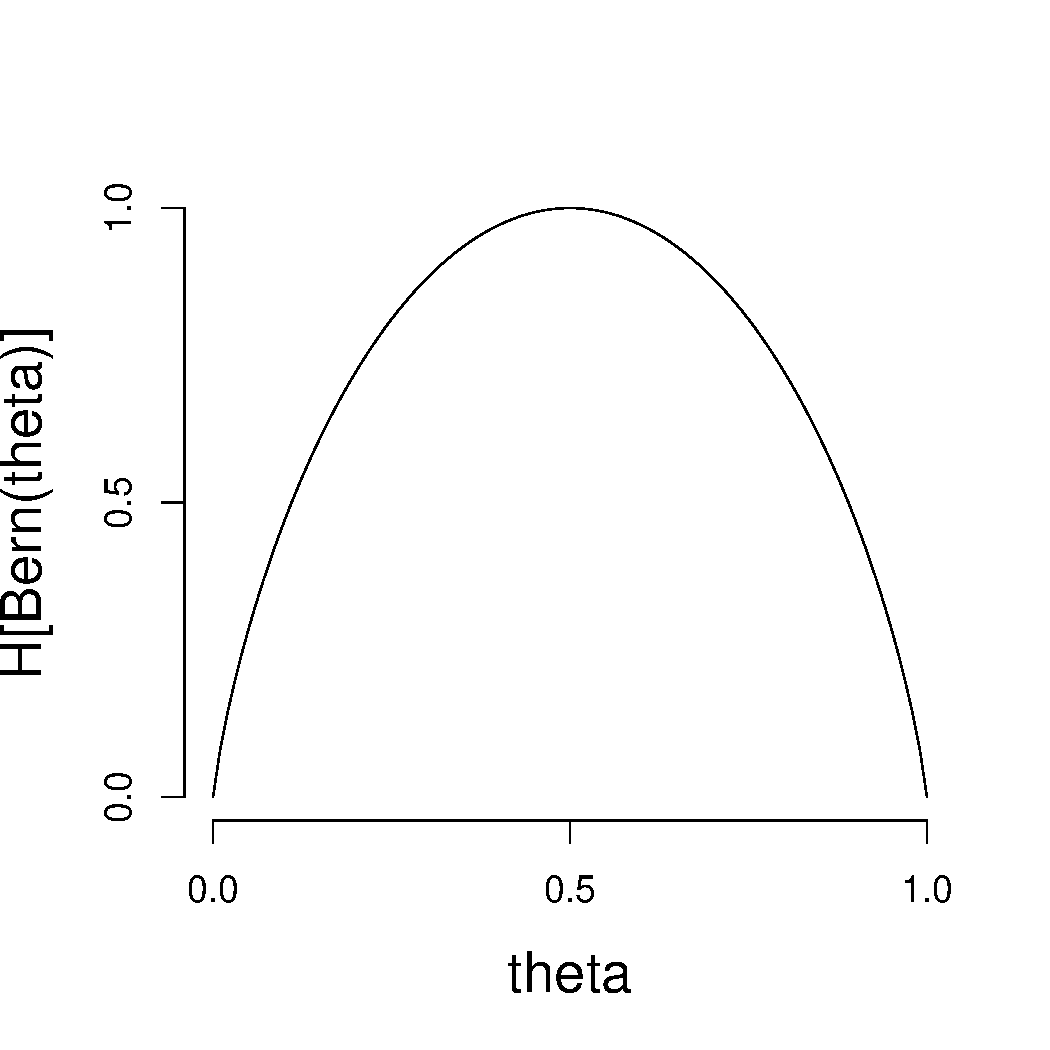
\includegraphics[height=1.75in]{pdfs/bern-entropy.pdf}
\end{center}%
\vspace*{-18pt}
\caption{Entropy of a random variable distributed as $\dbern{\theta}$.}\label{fig:bern-entropy}
\end{figure}
%
The graph makes it clear that when $\theta=0$ or $\theta=1$, the
outcome is certain, and therefore the entropy is 0.  The maximum
entropy possible for a Bernoulli distribution is 1 bit, achieved at
$\theta = 0.5$.  


\subsubsection{Entropy and Compression}

Entropy has a natural interpretation in terms of compression.  Suppose
we want to send the a message $X$ which might take on values in
$\nats$.%
%
\footnote{We can always code sequences of characters as numbers, as
originally noted by Kurt G\"odel, and as explained in any introductory
computer science theory text.  Just think of a string as representing
a number in the base of the number characters.}
%
If the sender and receiver both know the distribution $p_X$
of outcomes, the expected cost to send the message is $\entropy{X}$
bits.  For instance, if we need to send a bit with value 0 or 1, and
each outcome is equally likely, it will require 1 bit to send the
message.  On the other hand, if one outcome is more likely than the
other, we can save space (if we have repeated messages to send;
otherwise, we must round up).


\subsection{Joint Entropy}\label{section:stats-joint-entropy}

We can measure the entropy of two variables $X$ and $Y$ by measuring
the entropy of their joint distribution $p_{X,Y}$, generalizing our
definition to
%
\begin{equation}
\entropy{X,Y} = \expect{\log_2 p_{X,Y}(x,y)}.
\end{equation}
%
For instance, with discrete $X$ and $Y$, this works out to
%
\begin{equation}
\entropy{X,Y} = - \sum_{x} \sum_{y} p_{X,Y}(x,y) \ \log_2 p_{X,Y}(x,y).
\end{equation}
%

Joint entropy is symmetric, so that
%
\begin{equation}
\entropy{X,Y} = \entropy{Y,X}.
\end{equation}

\subsection{Conditional Entropy}\label{section:stats-conditional-entropy}

We can measure the entropy of a variable $X$ conditional on knowing
the value of another variable $Y$.  The expectation-based definition
is thus 
%
\begin{equation}
\condentropy{X}{Y} = \expect{-\log_2 p_{X|Y}(X|Y)}.
\end{equation}
%
In the case of discrete $X$ and $Y$, this works out to
%
\begin{align}
\condentropy{X}{Y} 
&= - \sum_y \sum_x p_{X,Y}(x,y) \ \log_2 p_{X|Y}(x|y)
\\
&= - \sum_y p_Y(y) \sum_x p_{X|Y}(x|y) \ \log_2 p_{X|Y}(x|y).
\end{align}
%

Conditional entropy, joint entropy and entropy are related as for
probabilty distributions, with
%
\begin{equation}
\entropy{X,Y} = \condentropy{X}{Y} + \entropy{Y}.
\end{equation}


\subsection{Mutual Information}\label{section:stats-mutual-information}

The mutual information between a pair of variables $X$ and $Y$ measures how
much more information there is in knowing their joint distribution than their
individual distributions for prediction.  Using expectations, mutual information
between variables $X$ and $Y$ is defined to be
%
\begin{align}
\mutualinfo{X}{Y} 
&= \expect{-\log_2 \frac{p_{X,Y}(x,y)}{p_X(x) \ p_Y(y)}}
\\
&= \expect{-\log_2 p_{X,Y}(x,y)} + \expect{\log_2 p_X(x)} + \expect{\log_2 p_Y(y)}
\end{align}
%
In the discrete case, this unfolds to
%
\begin{equation}
\mutualinfo{X}{Y} = - \sum_{x,y} p_{X,Y}(x,y) \ \log_2 \frac{p_{X,Y}(x,y)}{p_X(x) \ p_Y(y)}.
\end{equation}
%

Mutual information is symmetric, so that
%
\begin{equation}
\mutualinfo{X}{Y} = \mutualinfo{Y}{X}.
\end{equation}
%
It's related to conditional and joint entropies by the unfolding
in the second step of the definition through
%
\begin{align}
\mutualinfo{X}{Y} &= \entropy{X} + \entropy{Y} - \entropy{X,Y}
\\
&= \entropy{X} - \condentropy{X}{Y}.
\end{align}
%

\subsection{Cross Entropy}\label{section:stats-cross-entropy}

Cross-entropy measures the number of bits required, on average, to
transmit a value of $X$ using the distribution of $Y$ for coding.
Using expectation notation, the definition reduces to
%
\begin{equation}
\xentropy{X}{Y} = \expect{-\log_2 p_Y(X)}.
\end{equation}

In the case of discrete random variables $X$ and $Y$, this works out to
%
\begin{equation}
\xentropy{X}{Y} = - \sum_n p_X(n) \ \log_2 p_Y(n).
\end{equation}
%



\subsection{Divergence}\label{section:stats-divergence}

Kullback-Leibler (KL) divergence is the standard method to compare two
distributions.  Pairs of distributions that have similar probabilities
will have low divergence from each other.  Because KL divergence is
not symmetric, we also consider two standard symmetric variants.

Following the standard convention, our previous infomration
definitions were all in terms of random variables $X$ and $Y$, even
though the definitions only dependeded on their corresponding
probability distributions $p_X$ and $p_Y$.  Divergence is
conventionally defined directly on distributions, mainly to avoid the
case of comparing two different random variables $X$ and $Y$ with the
same distribution $p_X = p_Y$.

\subsubsection{KL Divergence}

Given two discrete distributions $p_X$ and $p_Y$, the KL divergence of
$p_Y$ from $p_X$ is given by
%
\begin{equation}
\kld{p_X}{p_Y}
= \sum_{n=1}^N p_X(n) \log_2 \frac{p_X(n)}{p_Y(n)}.
\end{equation}
%
If there is an outcome $n$ where $p_Y(n) = 0$ and $p_X(n) > 0$, the
divergence is infinite.  We may allow $p_X(n) = 0$ by interpreting $0
\log_2 \frac{0}{p_Y(n)} = 0$ by convention (even if $p_Y(n) > 0$).

If we assume $p_X$ and $p_Y$ arose from random variables $X$ and $Y$,
KL divergence may expressed using expectations as
%
\begin{align}
\kld{p_X}{p_Y} 
&= \expect{\log_2 \frac{p_X(X)}{p_Y(X)}}
\\
&= \expect{\log_2 p_X(X)} - \expect{\log_2 p_Y(X)}
\\
&= \expect{-\log_2 p_Y(X)} - \expect{-\log_2 p_X(X)}
\\
&= \xentropy{X}{Y} - \entropy{X}.
\end{align}
%
This definition makes clear that KL divergence may be viewed as as the
expected penalty in bits for using $p_Y$ to transmit values drawn from
$X$ rather than $p_X$ itself.  In other words, KL divergence is just
the cross-entropy minus the entropy.

Although we do not provide a proof, we note that $\kld{p_X}{p_Y} \geq 0$
for all distributions $p_X$ and $p_Y$.  We further note without proof
that $\kld{p_X}{p_Y} = 0$ if and only if $p_X = p_Y$.


\subsubsection{Symmetrized KL Divergence}\label{section:stats-symmetrized-kl-divergence}

KL divergence is not symmetric in the sense that there exist pairs of
random variables $X$ and $Y$ such that $\kld{p_X}{p_Y} \neq \kld{p_Y}{p_X}$.

There are several divergence measures derived from KL divergence that
are symmetric.  The simplest approach is just to introduce symmetry by
brute force.  The symmetrized KL-divergence $\skld{p_X}{p_Y}$ between
distributions $p_X$ and $p_Y$ is defined by averaging the divergence
of $p_X$ from $p_Y$ and the divergence of $p_Y$ from $p_X$, yielding
gives us
%
\begin{equation}
\skld{p_X}{p_Y} = \frac{1}{2}(\kld{p_X}{p_Y} + \kld{p_Y}{p_X}).
\end{equation}
%
Obviously, $\skld{p_X}{p_Y} = \skld{p_Y}{p_X}$ by definition, so the
measure is symmetric.  As with KL divergence, symmetrized KL
divergence so that, in general, $\skld{p_X}{p_Y} \geq 0$ with
$\skld{p_X}{p_Y} = 0$ if and only if $p_X = p_Y$.

\subsubsection{Jensen-Shannon Divergence}

Another widely used symmetric divergence measure derived from KL divergence
is the Jensen-Shannon divergence.  To compare $X$ and $Y$ using Jensen-Shannon
divergence, we first define a new distribution $p_{Z}$ by averaging
the distributions $p_X$ and $p_Y$, by
%
\begin{equation}\label{eq:jensen-shannon-averge-distro}
p_Z(n) = \frac{1}{2}(p_X(n) + p_Y(n)).
\end{equation}
%
If $X$ and $Y$ are random variables and $Z$ is defined to be
$(X+Y)/2$, then $p_X$, $p_Y$ and $p_Z$ satisfy the above definition.

Given the average distribution $p_Z$, we can define Jensen-Shannon
divergence by taking average divergence of $p_X$ and $p_Y$ from $p_Z$
as defined in \refeq{jensen-shannon-averge-distro}, setting
%
\begin{equation}
\jsd{p_X}{p_Y} = \frac{1}{2}(\kld{p_X}{p_Z} + \kld{p_Y}{p_Z}).
\end{equation}
%
As with the symmetrized KL divergence, Jensen-Shannon divergence is
symmetric by definition.


\subsubsection{LingPipe KL-Divergence Utilities}

KL-divergence is implemented as a static utility method in the
\code{Statistics} utility class in package \code{com.aliasi.stats}.
The method takes two double arrays representing probability
distributions and measures how much the first is like the second.

In order to give you a sense of KL-divergence, we implement a simple
utility in the demo class \code{KlDivergence} to let you try various
values.  The code just parses out double arrays from teh command line
and sends them to the KL function.
%
\codeblock{KlDivergence.1}

The ant target \code{kl} runs the command with the first two arguments
given by properties \code{p.x} and \code{p.y}.  To calculate the example
from above, we have
%
\commandlinefollow{ant -Dp.x="0.2 0.8" -Dp.y="0.4 0.6" kl}
\begin{verbatim}
pX=(0.2, 0.8)     pY=(0.4, 0.6)     
kld=0.13202999942307514    
skld=0.1415037499278844   
jsd=0.03485155455967723
\end{verbatim}
%
The Jensen-Shannon divergence is less than the symmetrized KL
divergence because the interpolated distribution $p_Z$ is closer to
both of the original distributions $p_X$ and $p_Y$ than they are to
each other.

